
\centerline{\textbf{ \LARGE Number System, Real Number Representation}}

\begin{questyle}
    \question  In 2's complement addition, overflow  (GATE-2002)
    \begin{enumerate}
        \item is flagged whenever there is carry from sign bit addition
        \item cannot occur when a positive value is added to a negative value
        \item is flagged when the carries from sign bit and previous bit match
        \item both number have same sign and result has the opposite sign.
    \end{enumerate}

  \begin{oneparchoices}
    \choice         I
    \CorrectChoice  II and IV
    \choice         II and III
    \choice         III and IV
  \end{oneparchoices}
\end{questyle}

\begin{questyle}
  \question  What is the result of evaluating the following two expressions using three-digit
             floating point arithmetic with rounding?  (GATE-2004)

             (113. + -111.) + 7.51 \\
             113. + (-111. + 7.51) \\
  \begin{oneparchoices}
    \CorrectChoice  9.51 and 10.0
    \choice         10.0 and 9.51
    \choice         9.51 and 9.51
    \choice         10.0 and 10.0
  \end{oneparchoices}

  Hint : Most significant 3 digits will taken from the result. 3rd MSB will be rounded of based on (n+1)th digit.\\
  Hint : (-111. + 7.51) = (103.49) = 103

\end{questyle}

\begin{questyle}
  \question  In the IEEE floating point representation, the hexadecimal value 0 × 00000000 corresponds to  (GATE-2008)

  \begin{choices}
    \choice         the normalized value \(2^{-127}\)
    \choice         the normalized value \(2^{-126}\)
    \choice         the normalized value +0
    \CorrectChoice  the special value +0
  \end{choices}
\end{questyle}


\begin{questyle}
  \question  The decimal value 0.5 in IEEE single precision floating point representation has (GATE-2012).

  \begin{choices}
    \choice         fraction bits of 0's and exponent value of 0
    \CorrectChoice  fraction bits of 0's and exponent value of -1
    \choice         fraction bits of 1..0's and exponent value of 0
    \choice         no exact representation
  \end{choices}
\end{questyle}

\begin{questyle}
  \question  A number(A.B) has non fractional part(A) and fractional part(B). Consider following
            representation. Maximum value that can be represented is \fillin[(\( 2^{n+f}\) -- 1)\( 2^{-f}\)] or
            \fillin[(\( 2^{n}\) -- \( 2^{-f}\))]. (Q made by me)
    \begin{center} 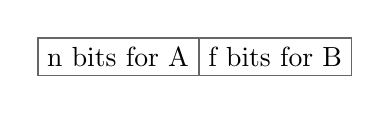
\begin{tikzpicture}[ baseline=0]
    \matrix [draw=white,column sep=0cm]
    {
        \node[draw=black!60] {n bits for A}; & \node[draw=black!60]{f bits for B}; \\
    };
    \end{tikzpicture} \end{center}
\end{questyle}

\begin{questyle}
  \question  The n-bit fixed-point representation of an unsigned real number X uses f bits for the
             fraction part. Let \mbox{i = n – f}. The range of decimal values for X in this representation is  (GATE-2017\_Set\_1)

  \begin{oneparchoices}
    \choice         \( 2^{-f}\)
    \choice         \( 2^{-f}\) to (\( 2^{i}\) -- \( 2^{-f}\))
    \choice         0 to \( 2^{-i}\)
    \CorrectChoice  0 to (\( 2^{i}\) -- \( 2^{-f}\))
  \end{oneparchoices}
\end{questyle}

\begin{questyle}
  \question  Given the following binary number in 32 bit (single precision) IEEE-754 format.
             The decimal value closest to this floating-point number is. (GATE-2017\_set\_2)

  \begin{choices}
    \choice         1.45 X \(10^1\)
    \choice         1.45 X \(10^{-1}\)
    \CorrectChoice  2.27 x \(10^{-1}\)
    \choice         2.27 x \(10^{1}\)
  \end{choices}
\end{questyle}

\begin{questyle}
  \question  Sign extension is a step in  (GATE-2002)

  \begin{choices}
    \choice         floating point multiplication
    \choice         signed 16 bit integer addition
    \choice         arithmetic left shift
    \CorrectChoice  converting a signed integer from one size to another
  \end{choices}
\end{questyle}

\begin{questyle}
  \question  The following is a scheme for floating point number representation using 16 bits.
             Let s,e, and m be the numbers represented in binary in the sign, exponent, and mantissa
             fields respectively. Then the floating point number represented is: (GATE-2003)

            \begin{center} 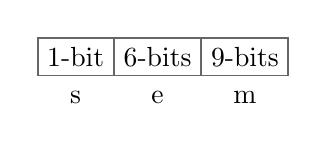
\begin{tikzpicture}[ baseline=0]
            \matrix [draw=white,column sep=0cm,row sep=0.07cm]
            {
                \node[draw=black!60] {1-bit}; & \node[draw=black!60]{6-bits}; & \node[draw=black!60] {9-bits}; \\
                \node[draw=white!60] {s}; & \node[draw=white!60]{e}; & \node[draw=white!60] {m}; \\
            };
            \end{tikzpicture} \end{center}

             What is the maximum difference between two successive real numbers representable in this system?
  \begin{oneparchoices}
    \choice         \(  2^{-40} \)
    \choice         \(  2^{-9} \)
    \CorrectChoice  \(  2^{22} \)
    \choice         \(  2^{31} \)
  \end{oneparchoices}
\end{questyle}

\begin{questyle}
  \question  Consider the following floating point format. Mantissa is a pure fraction in
             sign-magnitude form. (GATE-2005)

            \begin{center} 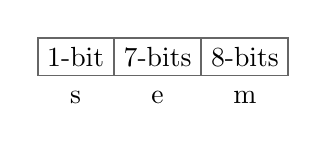
\begin{tikzpicture}[ baseline=0]
            \matrix [draw=white,column sep=0cm,row sep=0.07cm]
            {
                \node[draw=black!60] {1-bit}; & \node[draw=black!60]{7-bits}; & \node[draw=black!60] {8-bits}; \\
                \node[draw=white!60] {s}; & \node[draw=white!60]{e}; & \node[draw=white!60] {m}; \\
            };
            \end{tikzpicture} \end{center}

    \begin{parts}

    \part The decimal number 0.239 × \(2^{13}\) has the following hexadecimal
             representation (without normalization and rounding off).

    \begin{oneparchoices}
        \choice         0D 24
        \choice         0D 4D
        \choice         4D 0D
        \CorrectChoice  4D 3D (0 \; 1001101 \; 00111101)
    \end{oneparchoices}
    \\ Hint : 0.239 × \(2^{13}\) =  0.00111101 x \(2^{13}\)
    \\ Hint : e = 13+64 = 77 = 1001101, \quad m = 0.00111101

    \part The normalized representation for the above format is specified as follows. The mantissa has an implicit 1 preceding the binary (radix) point. Assume that only 0’s are padded in while shifting a field. The normalized representation of the above number 0.239 × \(2^{13}\)

    \begin{oneparchoices}
        \choice         0A 20
        \choice         11 34
        \choice         4D D0
        \CorrectChoice  4A E8 (0 \; 1001101 \; 00111101)
    \end{oneparchoices}
    \\ Hint : 0.239 × \(2^{13}\) =  0.00111101 x \(2^{13}\) = 1.11101 x \(2^{10}\)
    \\ Hint : e = 10+64 = 74 = 1001010,  \quad m = .11101 = .11101000

  \end{parts}
\end{questyle}

\begin{questyle}
  \question  The value of a float type variable is represented using the single-precision 32-bit
             floating point format IEEE-754 standard that uses 1 bit for sign, 8 bits for biased
             exponent and 23 bits for mantissa. A float type variable X is assigned the decimal value
             of -14.25. The representation of X in hexadecimal notation is  (GATE-2014\_set\_2)

  \begin{oneparchoices}
    \CorrectChoice  C1640000H
    \choice         416C0000H
    \choice         41640000H
    \choice         C16C0000H
  \end{oneparchoices}
    \\ Hint : -14.25 =  1110.01 = 1.11001 x \(2^{3}\)
    \\ Hint : e = 3 + 127 = 130 = 10000010,  \quad m = 0.110010.....0 (Total 23 bits)
\end{questyle}
